\chapter {Testing \& Results of Support Vector Classification}

\section{Classification of Testing Data}
To determine optimal performance, we wanted to test the system setup with different numbers of training points. Variable number of parameters were extracted from the image to test the improvement in performance of the SVM classification.

The testing data was gathered by hand, and later automated for ease of testing. After gathering the points they were classified into their respective categories with a premade mask selecting whether specific points were part of the door or not.

\section{Overall Effect}

Over the numerous types of parameters we could specify for the support vector machine to operate on, the order of effectiveness can be determined by the relative accuracy increase through its inclusion into the training data.

\\
The main parameters tested were as follows:

\begin{description}
  \item L*ab (Direct Pixel Value)
  \item L*ab (Radial Blur Pixel Value)
  \item XY (Pixel Location)
\end{description}


\begin{figure}
        \centering
        \begin{subfigure}[b]{0.3\textwidth}
                \centering
                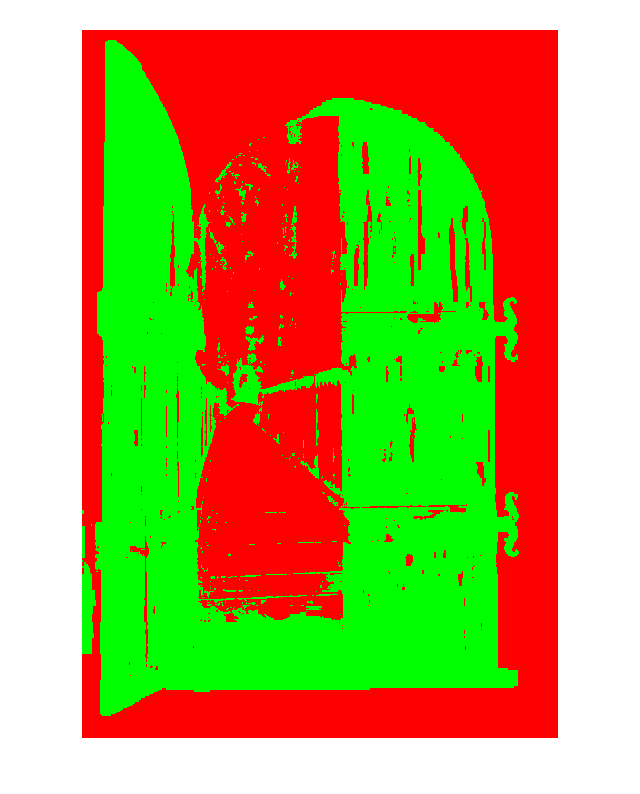
\includegraphics[width=\textwidth]{14_labtrainingonly}
                \caption{L*ab Pixel data}
                \label{fig:14_labtrainingonly}
        \end{subfigure}%
        ~ %add desired spacing between images, e. g. ~, \quad, \qquad etc.
          %(or a blank line to force the subfigure onto a new line)
        \begin{subfigure}[b]{0.3\textwidth}
                \centering
                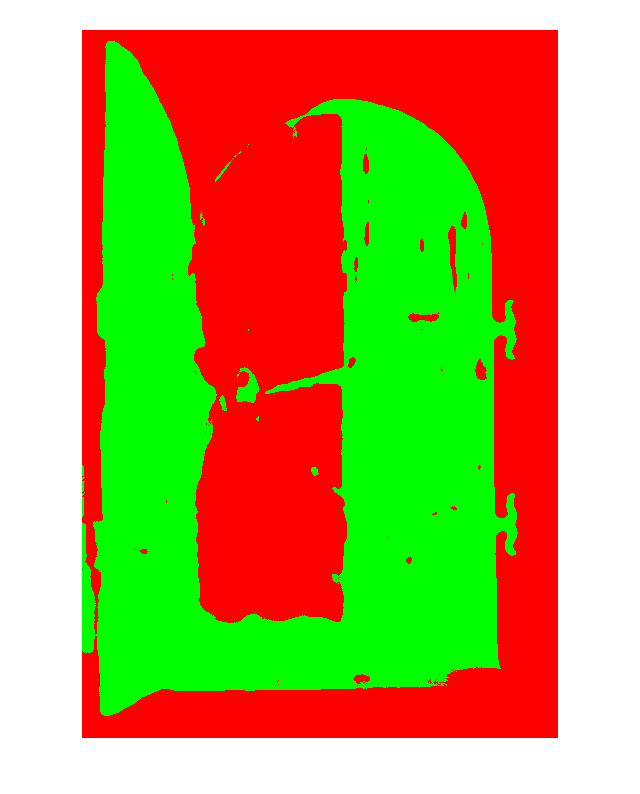
\includegraphics[width=\textwidth]{15_gaussianlabtrainingonly}
                \caption{L*ab Radial Blur}
                \label{fig:15_gaussianlabtrainingonly}
        \end{subfigure}
        ~ %add desired spacing between images, e. g. ~, \quad, \qquad etc.
          %(or a blank line to force the subfigure onto a new line)
        \begin{subfigure}[b]{0.3\textwidth}
                \centering
                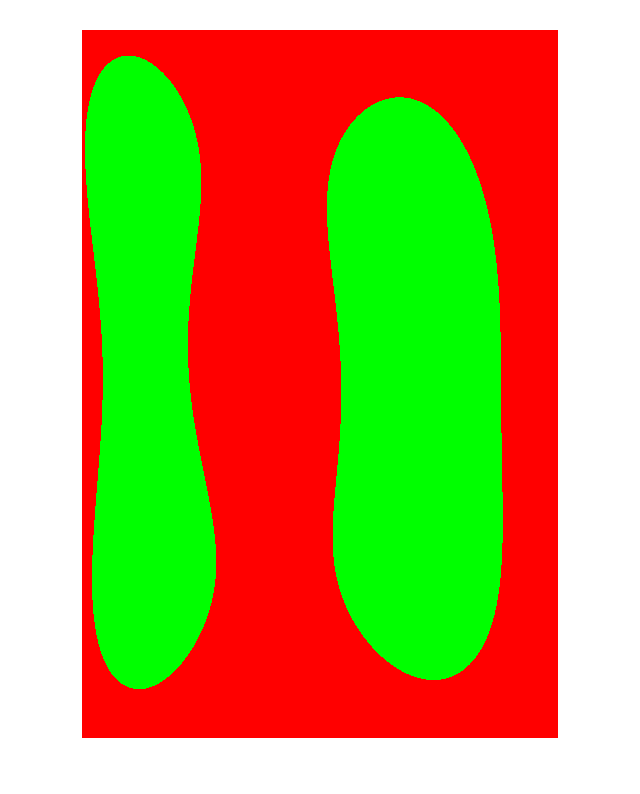
\includegraphics[width=\textwidth]{13_xytrainingonly}
                \caption{XY Pixel Location}
                \label{fig:13_xytrainingonly}
        \end{subfigure}
        \caption{Results of Differing SVM information, individual testing}\label{fig:labResults}
\end{figure}
The pixel location had a surprisingly opposite reaction to the effectiveness of the system upon adding its values to the training data. Using only the pixel coordinates to train the system had detrimental effects on the performance of the SVM. 

Seen in figure \ref{fig:labResults}, the hardest parts for the SVM to properly classify were the places with both similar colour and texture to the door. In these areas, the SVM had a higher probability to return false positive results.

In the end it was determined that the inputs that yielded the most optimal results were the L*ab colour data, the Sobel filter data, and the Gaussian Radial Blur. In effect, the pixel colour, the derivation, and the integration of the pixel value. This was done in an attempt to maximize the amount of information, without adding too many inputs to keep complexity too high.

\newpage

\section{Outcome}

\begin{figure}[ht]
    \centering
    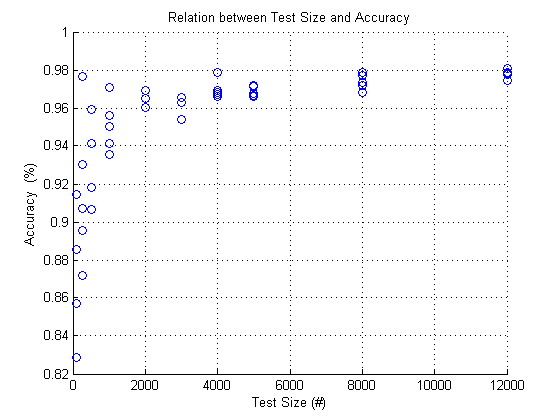
\includegraphics[height=3.5in]{12_testsizevsaccuracy}
    \caption{Changes in accuracy in the SVM from variance in the training set size.}
    \label{fig:12_testsizevsaccuracy}
\end{figure}

By limiting the data sent to the training set for the support vector machine, it was possible to observe 90\% and above performance for even small amounts of training data. The position of these points had a greater effect on the results than when the number of points was higher. The variance in the accuracy with differing test sets decreased when the total number of points increased. As expected, the results are very sensitive to the position of the training points; more points will become support vectors that are further away from the optimal hyperplane.
\\







